% Clean I3M/EMSS submission manuscript.
\documentclass[3p,times,procedia]{elsarticle}
\flushbottom

\usepackage{ecrc}
\usepackage{amsmath}
\usepackage{amssymb}
\usepackage{booktabs}
\usepackage{graphicx}
\usepackage[bookmarks=false]{hyperref}

\hypersetup{colorlinks,linkcolor=blue,citecolor=blue,urlcolor=blue}

\volume{00}
\firstpage{1}
\journalname{Procedia Computer Science}
\runauth{Tong and Zhao}
\jid{procs}
\graphicspath{{figures/}}

\begin{document}
\begin{frontmatter}

\dochead{38th European Modeling \& Simulation Symposium (EMSS 2026), I3M 2026}

\title{A Controlled-Replay Prototype for Auditable Versioned Financial Event Graph Updates}

\author[a]{Jiakai Tong}
\author[a]{Yue Zhao}
\address[a]{School of Astronautics, Harbin Institute of Technology, Harbin, China}

\begin{abstract}
Financial event records used in simulation and audit workflows require evidence links, update histories, and reproducible state transitions. This paper presents a controlled-replay prototype for auditable versioned financial event graph updates. The artifact checks required event-record fields, enforces exact evidence-span containment, applies deterministic graph update operators, and records append-only version logs. Evaluation is intentionally narrow: 70 controlled records exercise oracle-controlled replay, a metadata-hidden diagnostic obtains 0.586 operator agreement, 20 FewFC-derived public mini-case records provide an external sanity check, and a 560-record scale sanity run checks lightweight runtime behavior. The paper reports no extraction F1, no market prediction, and no benchmark-level generalization. The evidence supports a limited auditability claim: controlled financial event updates can be replayed into inspectable graph transitions with explicit evidence and failure logs.
\end{abstract}

\begin{keyword}
event graph \sep controlled replay \sep discrete-event simulation \sep auditability \sep version log
\end{keyword}

\end{frontmatter}

\clearpage

\section{Introduction}

Financial event records are often treated as final structured outputs. For modeling and simulation workflows, that view is incomplete: a record may duplicate a prior disclosure, revise a previous amount, or contradict an earlier statement. If such changes are silently overwritten, later audit and verification become difficult. A simulation artifact should therefore preserve evidence, replay order, state transitions, and failure reasons.

Event records need replay and version logs because their operational meaning depends on graph state. The same incoming record may be a new event in an empty graph, a merge candidate after a target exists, or a failed operation if target resolution cannot be justified. A compact replay model can make these decisions inspectable by connecting each accepted record to a graph transition and each rejected record to an explicit skip reason.

Existing financial event extraction research focuses on converting documents into structured events \cite{yang2018dcfee,zheng2019doc2edag,ma2022fewfc}. Provenance and event-sourcing work emphasizes traceable state reconstruction \cite{w3c2013provo,fowler2005eventsourcing}. Discrete-event simulation and verification literature emphasizes explicit event-driven state change and validation discipline \cite{banks2010discrete,law2015simulation,sargent2013verification}. The gap addressed here is narrower: a reproducible artifact for evidence-gated replay of controlled financial event records into a versioned event graph.

This paper makes three contributions. First, it defines an evidence-gated controlled replay model for financial event records. Second, it implements versioned event graph transition artifacts, including target resolution, invariant checks, version logs, and replay traces. Third, it reports reproducible diagnostics, including metadata-hidden replay, negative controls, invariant checks, a public mini-case, and a scale sanity run.

\section{Related work}

\subsection{Financial event extraction and event records}

Document-level financial event extraction systems such as DCFEE \cite{yang2018dcfee} and Doc2EDAG \cite{zheng2019doc2edag} show that financial events often require multi-sentence argument assembly. FewFC provides a public few-shot financial event extraction dataset \cite{ma2022fewfc}. These works motivate structured financial event records. The present artifact starts after record construction and studies replay, evidence gates, and graph update logs rather than extraction model quality.

\subsection{Provenance, audit trails, and event sourcing}

The W3C PROV-O vocabulary defines provenance concepts for entities and activities \cite{w3c2013provo}. Event sourcing records state changes as an append-only event history \cite{fowler2005eventsourcing}. Database and workflow audit trails similarly emphasize traceable data evolution \cite{buneman2001and}. The prototype follows this auditability principle in a compact graph setting: each applied or failed replay decision is represented as a version log entry.

\subsection{Discrete-event simulation and reproducible artifacts}

Discrete-event simulation describes systems whose state changes at event times \cite{banks2010discrete,law2015simulation}. Verification, validation, and testing guidance for simulation models stresses traceable assumptions, reproducible runs, and explicit limits on interpretation \cite{sargent2013verification}. This paper uses those ideas for event graph maintenance: incoming records trigger state transitions, while replay traces support inspection and reproduction.

\section{Methodology}

\subsection{Event records and evidence gate}

An event record is represented as
\begin{equation}
x_i = (id_i, type_i, subj_i, obj_i, time_i, trig_i, span_i, doc_i, text_i, a_i, status_i).
\end{equation}
The required fields are event identity, event type, subject, object, date, trigger, evidence span, source document identifier, and source text. Optional slots include amount and status. A record passes the evidence gate only when
\begin{equation}
span_i \ne \emptyset \quad \wedge \quad span_i \subset text_i,
\end{equation}
where containment is exact string containment. The main experiments do not use fuzzy matching.

\subsection{Replay policy and target resolution}

At replay step $t$, the simulator chooses an operator
\begin{equation}
o_t \in \{\texttt{ADD\_EVENT}, \texttt{MERGE\_EVENT}, \texttt{UPDATE\_SLOT}, \texttt{MARK\_CONFLICT}\}.
\end{equation}
The oracle-controlled policy may read controlled metadata: perturbation type, expected operator, and base event identifier. The rule-based policy may read only event fields and current graph state. It cannot use perturbation labels, expected operators, gold grouping fields, or a direct base identifier as a target shortcut.

Target resolution is also split. Oracle target selection may use a base identifier only if that target exists in the graph. Rule-based target selection uses subject, event type, date proximity, amount, status, and textual update or conflict cues. If no target exists for a target-dependent operator, replay returns no target and records a failed operation.

\subsection{Invariant checks and graph transition}

The graph state is
\begin{equation}
G_t = (V_t, E_t, L_t),
\end{equation}
where $V_t$ contains event and entity nodes, $E_t$ contains event-entity links, and $L_t$ is an append-only version log. The transition is
\begin{equation}
G_t \xrightarrow{o_t} G_{t+1}.
\end{equation}
The simulator also records a compact state summary
\begin{equation}
S_t = (g_t, n^e_t, n^v_t, n^m_t, n^u_t, n^c_t, n^{uc}_t),
\end{equation}
where the terms denote graph version, active events, active entities, successful merges, successful slot updates, conflict marks, and unresolved conflicts. Failed target resolution is logged with \texttt{operation\_applied=false}; it does not increment successful merge, update, or unresolved conflict counts.

\subsection{Version log schema}

Each version log entry stores the replay step, graph version, operator, incoming event identifier, target identifier when available, target-existence flag, applied flag, skip reason, source document identifier, and operation details. Unsupported metadata is logged with \texttt{skipped\_reason=unsupported\_or\_unknown\_metadata}.
Figure~\ref{fig:workflow} summarizes the replay workflow, and Figure~\ref{fig:transition} shows the state-transition view used by the simulator.

\begin{figure}[t]
\centering
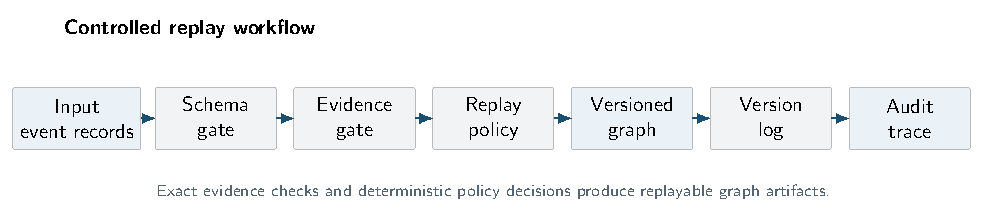
\includegraphics[width=0.96\hsize]{fig_workflow.pdf}
\caption{Workflow for evidence-gated replay from event records to graph artifacts and audit traces.}
\label{fig:workflow}
\end{figure}

\begin{figure}[t]
\centering
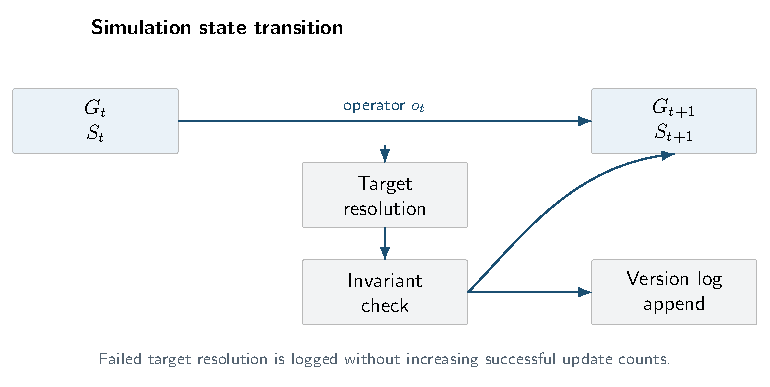
\includegraphics[width=0.94\hsize]{fig_state_transition.pdf}
\caption{State-transition view linking target resolution, invariant checks, graph update, and version-log append.}
\label{fig:transition}
\end{figure}

\section{Experiments}

\subsection{Controlled oracle replay}

The controlled stream contains 70 records derived from 30 deterministic seed records. It injects duplicate, update, conflict, and out-of-order replay perturbations. Table~\ref{tab:oracle-replay} reports schema validity, evidence coverage, replay completeness, and agreement with injected operator labels. These agreement values are controlled diagnostics, not extraction accuracy.

\begin{table}[t]
\caption{Controlled replay diagnostics; agreement compares replay decisions with injected operator labels, not extraction accuracy.}
\label{tab:oracle-replay}
\begin{tabular*}{\hsize}{@{\extracolsep{\fill}}lrrrrrrrr@{}}
\toprule
Method & Schema & Evidence & Merge & Conflict & Update & Operator & Replay & n\\
\midrule
Direct records & 1.000 & 1.000 & -- & -- & -- & -- & -- & 70\\
Schema gate & 1.000 & 1.000 & -- & -- & -- & -- & -- & 70\\
Evidence gate & 1.000 & 1.000 & -- & -- & -- & -- & 1.000 & 70\\
Oracle-controlled & 1.000 & 1.000 & 1.000 & 1.000 & 1.000 & 1.000 & 0.871 & 70\\
\bottomrule
\end{tabular*}
\end{table}


\subsection{Metadata-hidden rule-based replay}

The metadata-hidden diagnostic removes perturbation labels, expected operators, direct base identifiers, and gold grouping fields before policy decisions. Gold labels are restored only after replay to compute agreement. Table~\ref{tab:metadata-hidden} shows that the metadata-hidden operator agreement is 0.586, exposing the current rule limits.

\begin{table}[t]
\caption{Metadata-hidden diagnostic replay agreement.}
\label{tab:metadata-hidden}
\begin{tabular*}{\hsize}{@{\extracolsep{\fill}}llrrrrrr@{}}
\toprule
Setting & Metadata & Merge & Conflict & Update & Operator & Replay & Runtime\\
\colrule
Full-control & yes & 1.000 & 1.000 & 1.000 & 1.000 & 1.000 & 0.016\\
Metadata-hidden & no & 0.200 & 0.800 & 0.700 & 0.586 & 1.000 & 0.012\\
\botrule
\end{tabular*}
\end{table}


\subsection{Public mini-case}

The public mini-case uses 20 FewFC-derived records as an external sanity check only. It tests whether converted public financial event text can pass the same schema, exact evidence, and replay path. Table~\ref{tab:public-mini-case} reports this check. It is not a benchmark and does not report extraction F1.

\begin{table}[t]
\caption{Public-dataset mini-case external sanity check.}
\label{tab:public-mini-case}
\begin{tabular}{@{}lrrrrrrp{0.29\hsize}@{}}
\toprule
Dataset & Records & Schema & Evidence & Replay & Active events & Logs & Notes\\
\colrule
FewFC & 20 & 1.000 & 1.000 & 1.000 & 20 & 20 & external sanity case only; no extraction F1 or benchmark claim\\
\botrule
\end{tabular}
\end{table}


\subsection{Negative controls and invariant checks}

Negative controls include missing required fields, evidence mismatches, invalid dates, and unsupported metadata. Table~\ref{tab:negative-controls} reports rejection and logging behavior. Table~\ref{tab:invariant-checks} reports a separate small invariant check suite. These invariant checks verify that failed target resolution and unsupported metadata are logged without being counted as successful graph updates.

\begin{table}[t]
\caption{Negative controls verify rejection and logging paths without successful graph updates.}
\label{tab:negative-controls}
\begin{tabular*}{\hsize}{@{\extracolsep{\fill}}rrrrrr@{}}
\toprule
Cases & Schema rej. & Evidence rej. & Bad dates & Unsupported logged & Crashes\\
\midrule
20 & 10 & 5 & 5 & 5 & 0\\
\bottomrule
\end{tabular*}
\end{table}

\begin{table}[t]
\caption{Invariant checks for failed target resolution and unsupported metadata.}
\label{tab:invariant-checks}
\begin{tabular}{@{}p{0.21\hsize}p{0.34\hsize}lll@{}}
\toprule
Case & Expected behavior & Applied & Logged & Result\\
\midrule
Missing target merge\_event & log missing target without success count & false & true & pass\\
Missing target update\_slot & log missing target without success count & false & true & pass\\
Missing target mark\_conflict & log missing target without success count & false & true & pass\\
Invalid nested event & return schema error & false & true & pass\\
Unsupported metadata & log unsupported metadata without update & false & true & pass\\
Evidence mismatch & reject before graph update & false & true & pass\\
\bottomrule
\end{tabular}
\end{table}


\subsection{Scale sensitivity and case study}

The scale sanity run uses deterministic streams up to 560 replay records. Table~\ref{tab:scale} reports graph sizes and runtime per record, while Figure~\ref{fig:diagnostic-results} combines metadata-hidden agreement with runtime scaling. Table~\ref{tab:case-study} provides a short replay-trace excerpt.

\begin{table}[t]
\caption{Scale sanity run over deterministic controlled streams.}
\label{tab:scale}
\begin{tabular*}{\hsize}{@{\extracolsep{\fill}}rrrrrrr@{}}
\toprule
Seed records & Replay records & Active & Logs & Conflicts & Replay & ms/rec.\\
\midrule
30 & 70 & 40 & 70 & 7 & 0.871 & 0.024\\
60 & 140 & 80 & 140 & 14 & 0.864 & 0.039\\
120 & 280 & 160 & 280 & 31 & 0.896 & 0.030\\
240 & 560 & 320 & 560 & 63 & 0.920 & 0.028\\
\bottomrule
\end{tabular*}
\end{table}


\begin{figure}[t]
\centering
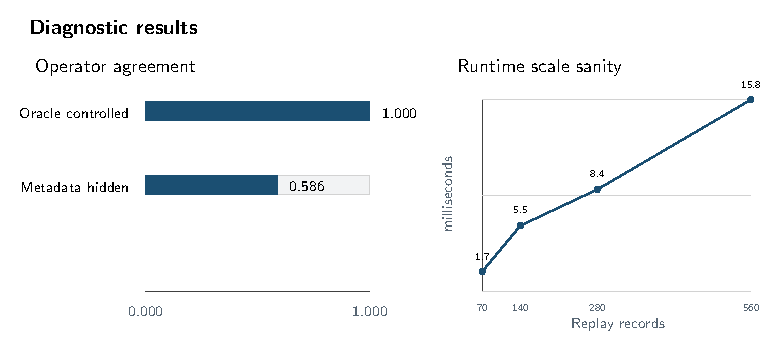
\includegraphics[width=0.96\hsize]{fig_diagnostic_results.pdf}
\caption{Diagnostic view of oracle-controlled versus metadata-hidden operator agreement and scale sanity runtime.}
\label{fig:diagnostic-results}
\end{figure}

\begin{table}[t]
\caption{Replay trace excerpt showing representative graph transitions.}
\label{tab:case-study}
\begin{tabular}{@{}rlp{0.28\hsize}p{0.34\hsize}@{}}
\toprule
Step & Operator & Event transition & Replay note\\
\midrule
1 & \texttt{ADD\_EVENT} & E000016 & accepted evidence-backed record\\
2 & \texttt{ADD\_EVENT} & E000007\_TS007 & accepted evidence-backed record\\
3 & \texttt{ADD\_EVENT} & E000007 & accepted evidence-backed record\\
19 & \texttt{MARK\_CONFLICT} & E000005\_CON005 -> E000005 & marked unresolved conflict\\
29 & \texttt{MERGE\_EVENT} & E000007\_DUP007 -> E000007 & merged duplicate into target\\
32 & \texttt{UPDATE\_SLOT} & E000003\_UPD003 -> E000003\_TS003 & updated changed slots\\
\bottomrule
\end{tabular}
\end{table}


\section{Discussion}

The oracle-controlled setting is an upper-bound sanity check because controlled metadata can identify intended operators and targets. It should not be read as deployment performance. The metadata-hidden result is more informative for method limits: it shows that simple rules recover part of the injected structure, but still miss many controlled operator labels.

The public mini-case is deliberately small and is used only to exercise the replay path on externally sourced text. The exact span gate is strict: it favors auditability and reproducibility over tolerant matching. The artifact reports no extraction F1 and no market prediction. It also does not implement human review, persistent graph storage, or large public-dataset replay. Future work should expand public replay coverage, add human review workflows for unresolved conflicts, and move the graph store to a durable backend.

\section{Conclusion}

This paper presented an evidence-gated controlled replay prototype for auditable versioned financial event graph updates. The artifact records schema checks, exact evidence containment, target resolution, graph transitions, invariant failures, and version logs. The evidence supports a narrow auditability claim: controlled financial event updates can be replayed into inspectable graph artifacts with explicit success and failure accounting.

\bibliographystyle{elsarticle-num}
\bibliography{references}

\end{document}
